{\textbf{基本思想:}}

{1. 先从数列中取出一个数作为基准数。}

{2.
分区过程,将比这个数大的数全放到它的右边,小于或等于它的数全放到它的左边。}

{3. 再对左右区间重复第2步,直到各区间只有一个数。}

{\textbf{代码如下:}}

{\textbf{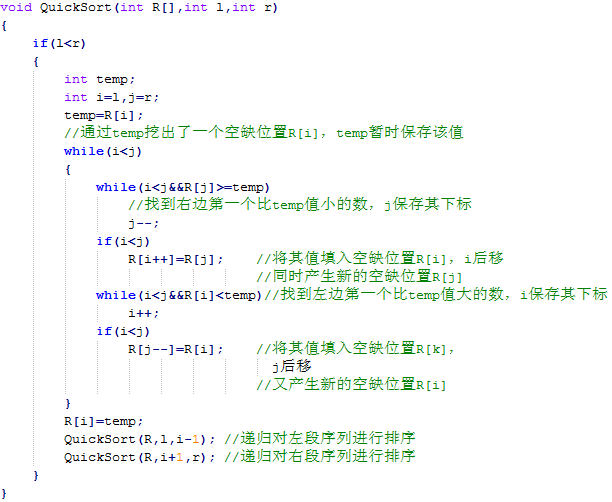
\includegraphics[width=3.70833in,height=3.04167in]{png-jpeg-pics/48AE513E40803512100E36ECD2D64C7E.png}\\
}}

{\textbf{算法分析:}}{快速排序的时间复杂度为O(nlog}\textsubscript{2}{n),快排在同为O(nlog}\textsubscript{2}{n)的几种排序方法中效率较高,}{快排的空间复杂度为}{O(log\textsubscript{2}n)}{,因为是递归函数,需要栈的辅助,分析不会考。}
